
% Currently supported format is the 4:3 aspect ratio (and not 16:9)
% You need to select the LuaTeX engine to compile to pdf
% If you use Overleaf, you have to change the compiler (https://www.overleaf.com/learn/how-to/Changing_compiler)
% Reason: The common pdfTeX engine cannot use system fonts: Calibri, Georgia

\documentclass[aspectratio=43]{beamer} %43 should be in fact the default

% Load package "amsmath" before PSI43 (because "fontspec" inside PSI43 should be loaded before "amsmath" according to an advice)
\usepackage{amsmath}

\usepackage[blockcolored]{PSI43} % blockcolored is required if you want to have colored blocks, because the default beamer theme has uncolored boxes







\begin{document}

\title{A novel approach to energy system analysis and technology assessment}

\author[L.~Wittgenstein]{Ludwig Wittgenstein}
% if short author is given as an option, it will be taken for the footline

\institute[LEA, PSI]{Laboratory of Energy Systems Analysis, Paul Scherrer Institute}
% if short institute is given as  an option, it will be taken for the footline

\subtitle{1st Line\\2nd Line (a 3rd line may be required for single-line titles to move gray box down)}

\date{LEA Seminar, 1.1.2021} % can be left empty

\begin{frame}[plain] % plain prohibits logo, footer etc.
  \titlepage
\end{frame}


\begin{frame}{A list that is reveiled}  
  \begin{itemize}
  \item<1-> Item 1
  \item[-]<1->  Item 1 (with dash instead of bullet)
    \begin{itemize}
    \item<1-> Item 1b
    \end{itemize}
  \item<2->  Item 2 (revealed on next slide)
  \item<3-> Item 3
    \begin{itemize}
    \item<3-> Item 4
      \begin{itemize}
      \item<3-> Item 5
      \end{itemize}
    \end{itemize}
  \end{itemize}
 \vspace*{\fill} % to put the text a little bit upwards
\end{frame}



\begin{frame}[squeeze]{Titles over two lines are possible (just the PSI logo is a little bit down)}
  Some formulas:
  \begin{align*}
    a + b  & = \int_a^b f(x)\,dx \\
    \sum_{n=1}^N x_{i_n} &= \frac{a+b}{c+d} 
  \end{align*}
  \begin{itemize}
  \item  $\alpha = \zeta$ 
  \item $\mathcal{F}_t$, $\mathbb{R}^n$
  \item $\{t \mid t=1,\dots,T\}$
  \item $f\colon x\to y$
  \end{itemize}
   \alert{This is a frame with the usual `squeeze' option of beamer to narrow linespacing a little bit, The color of this text is called ``alert'' in beamer}
  
  \structure{This is a color predefined in beamer called ``structure''}
\end{frame}

\begin{frame}{Columns and Blocks}
  You can start text very high with a space command (look into the .tex file of this presentation)

 The default beamer theme has uncolored blocks. An option was set for coloring: 
  \begin{columns}
    \begin{column}[T]{0.6\linewidth}
      \begin{block}{Text in a block}
        This is a block of text in the first column
      \end{block}
      \begin{exampleblock}{Text in an example block}
        This is a block of text in the first column
      \end{exampleblock}
      Text outside of block in first column
    \end{column}
    \begin{column}[T]{0.4\linewidth}
      \begin{block}{Text in a block}
        This is a block 
      \end{block}
      \begin{alertblock}{Text in an alert block}
        This is a block
      \end{alertblock}
      \begin{block}{}
        This is a block without title (not nice)
      \end{block}
    \end{column}
  \end{columns}
    
    \PSIfill
 \end{frame}
 

 \begin{frame}{Text}
   \PSIvspace
  You can start text at the gray box with a space command (see the .tex file)
  \begin{figure}
    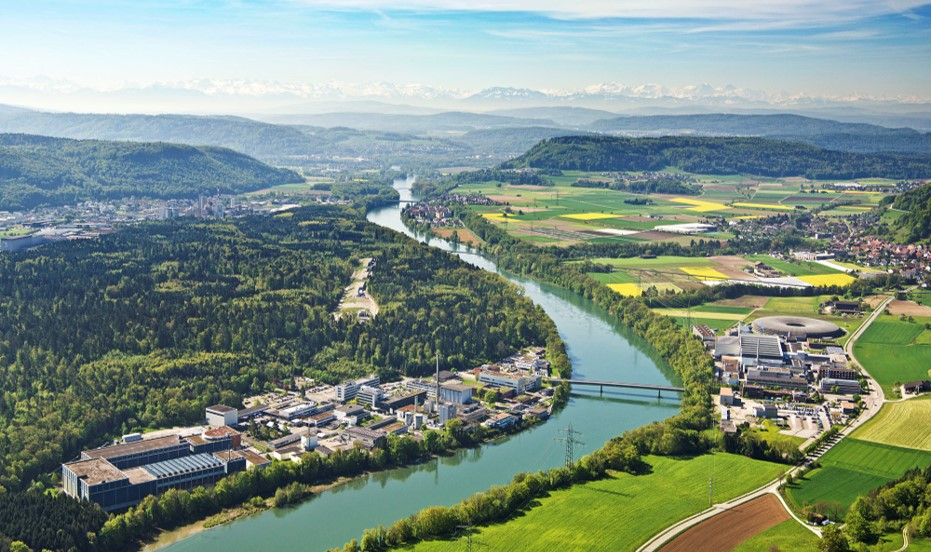
\includegraphics[width=0.3\pagewidth]{PSIlandscape}
    \caption{Figures are automatically centered in beamer}
    \label{fig:PSI}
    \end{figure}

     \PSIfill
\end{frame}

\begin{frame}{Overwrite the margins}
\begin{columns}
  \begin{column}{1.2\linewidth}
     If you need a lot of space, just use an oversized column, as in the code of this slide
     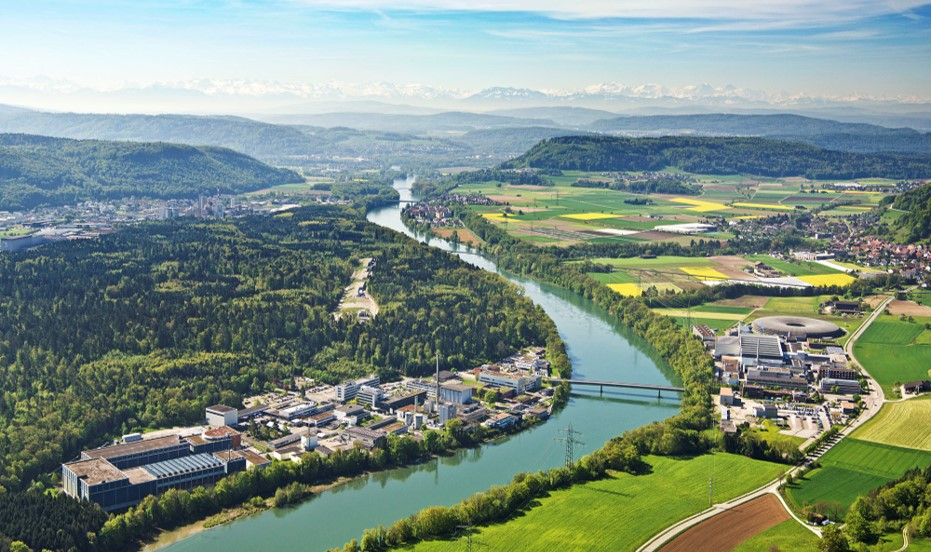
\includegraphics[width=12.5cm]{PSIlandscape}
  \end{column}
\end{columns}
\end{frame}

\PSItrailer{
    \textbf{My thanks go to}
     \smallskip
    \begin{itemize}
    \item Co-author 1
    \item Co-author 2 who has a very long name 
    \item Supervisor 1
    \item Supervisor 2  
    \end{itemize}
    }
  

\end{document}

% The following can be deleted if not the EMACS editor is used for editing

%%%Local Variables:
%%% mode: latex
%%% TeX-master: t
%%% TeX-engine: luatex
%%% End:
